\chapter{Introduction}
\label{chapter_1}

This chapter presents introduction about the host institution (namely ICTLab), the internship context, the internship objective and the report organization. 

%%%
\section{Context}

%%%
\subsection{Company Introduction}

%%% 
ICTLab, a joint international research laboratory about Information and Communication Technology (ICT), was created on December 2014 at Hanoi, Vietnam. It is an international collaboration between University of Science and Technology of Hanoi (USTH), Institute of Information Technology (IOIT) of Vietnamese Academy of Science and Technology (VAST), IRD (Institut de Recherche pour le Développement) and the University of La Rochelle, France~\cite{ictlab}.

The research program at the ICTLab of USTH targets various scientific axes, including Modeling and Simulation, Health Bioinformatics, High Performance Computing, Machine Learning, Data Mining, Image Processing, Computer Vision and Document Analysis. Beside doing research, ICTLab also hosts internships for bachelor, master and doctoral programs.

Corresponding to these research axes, ICTLab researchers are working on different research projects, namely SWARMS, ARCHIVES, GPU4SPACE and HealthOmics. 

%%%
\subsection{Internship context}

SWARMS (Say and Watch: Automated image/sound Recognition for Mobile monitoring Systems) is one of the 4 main projects at ICTLab. Its goal is to obtain a flexible and real-time monitoring network in order to feed decision support systems or support advanced visualization of the phenomenon to monitor~\cite{ictlab}. During the first year of its implementation, ICTLab researchers are in progress of building a dataset for SWARMS project. This dataset contains a set of digital images which were collected by sending USTH bachelor students to the fields and taking photos. 

This internship was happened in the context of SWARMS project where the goal is to improve the quality of image dataset collected by USTH bachelor students during their field trips. Since USTH bachelor students are not experts in photograpy, their taken photos may be added noise which, in turns, degrade the image by changing its brightness or its color information. Noise appearing in images represents unwanted components which degrades the image. It is the cause of errors from image when the pixel values do not reflect the true intensities of the real image scene. The noisy image may contain the information which is very different from the original normal image. 

One common type of noise, called random noise, may easily exist in SWARMS images. This random noise is created by camera sensors with high ISO values in short exposure. ISO is a popular photography metric which describes the sensor's absolute sensitivity to light. Higher ISO value increases sensor sensitivity (i.e. how quickly the sensor absorbs light), but also adds noise to the captured photo. In other words, students tried to give more light to the camera to create lighter image, but also makes more noise appear to the image, especially in low light conditions, such as dark places or in the evening.

Since the appearance of noise degrades quality of images, it reduces accurary of SWARMS systems and consequently reduces outcomes of the project. Therefore, it is necessary to remove noise from taken images in order to enhance performance of SWARMS systems. 

In this internship, we are going to study different image denoising techniques. The studied methods include Median filter, Average filter, Gaussian filter and Wiener filter. From these methods, we will compare their results by using two metrics: Mean Square Error (MSE) and Peak Signal to Noise Ratio (PSNR). Based on the quality characteristics of these two metrics, one efficient method is chosen to denoise the captured images for SWARMS project.

%%%
\section{Problematic}

\subsection{Noise and Types of Noise}

\textbf{Noise definition}
Noise is an unwanted component of the image which can be additive or multiplicative. A captured image $i(.)$ can be decomposed into two components: a desired component $d(.)$, and a noise component $n(.)$. In the literature there exists two popular noise models: additive model and mulitplicative model. 

The formula of the former is given by:

\begin{equation}
	i(.) = d(.) + n(.)
\end{equation}

Gaussian noise, quantization noise, poisson noise and uniform noise are examples of additive noise. 

The formula of the latter is as follows:

\begin{equation}
	i(.) = d(.)n(.)
\end{equation}

Speckle noise is an example of multiplicative noise. 

\textbf{Types of noise}

There exists many types of noise in images. In this internship, only common and basic types of noise are studied, including Salt and Pepper Noise, Gaussian Noise, Quantization Noise and Speckle Noise.

\textbf{Salt and Pepper Noise}, also called Impulse Noise, is a type of noise having dark pixels in bright regions and bright pixels in dark regions. Salt and Pepper Noise can be caused by sharp and sudden disturbances in the image signal, bit errors in transmission or errors in analog-to-digital conversion. 

The probability density function of salt and pepper noise is given as follows:

\begin{equation}
    f_{ps}(x)= 
\begin{cases}
    f_p, & \text{for } x = p\\
    f_s, & \text{for } x = s\\
    0,              & \text{otherwise}
\end{cases}
\end{equation}

where $f_p$ and $f_s$ are occurrence probabilities of pixels having values equal to $p$ (pepper) or $s$ (salt). These salt and pepper pixels are also called dead pixels of the image. Figure~\ref{fig:salt_pepper_noise} presents an example of image with salt and pepper noise compared to the original image.

\begin{figure}
    \centering 
    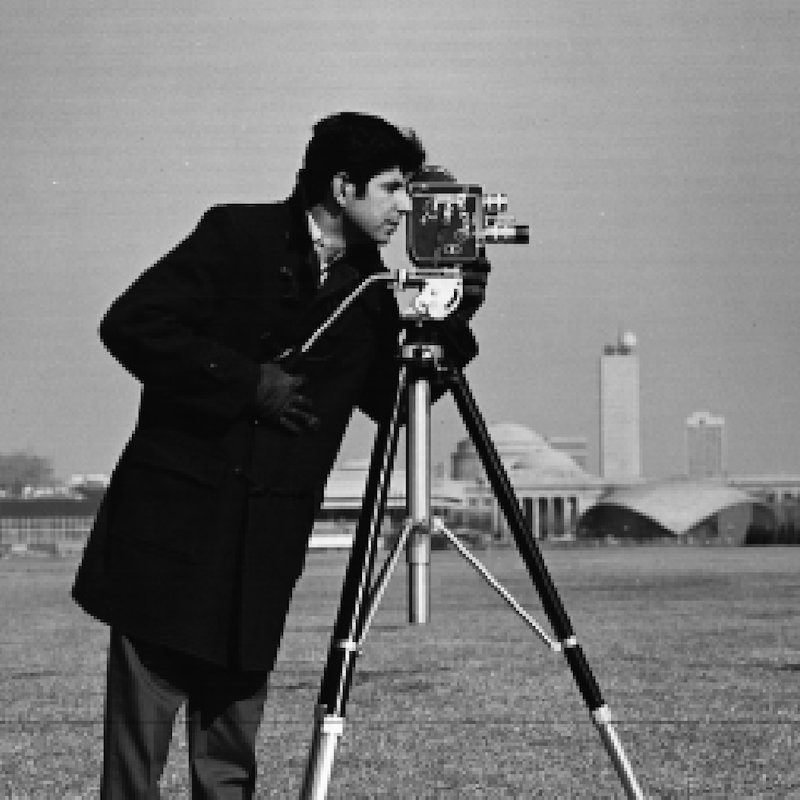
\includegraphics[width=0.4\columnwidth]{images/salt_pepper_origin.jpg}
    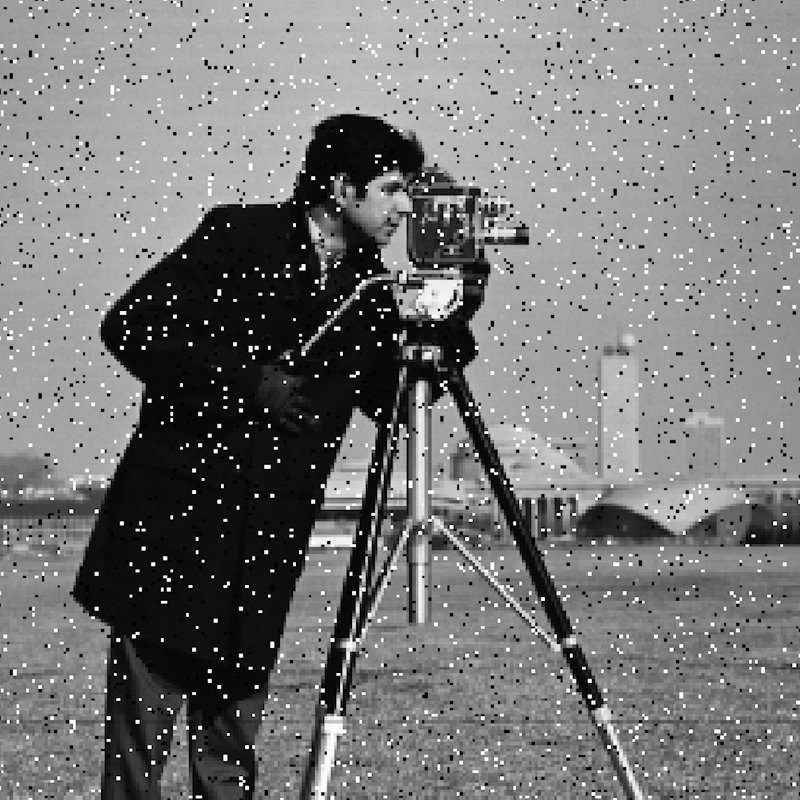
\includegraphics[width=0.4\columnwidth]{images/salt_pepper_noise.jpg}
	\caption{Original image (left column) and salt and pepper noise (right column).}
	\label{fig:salt_pepper_noise}
\end{figure}

%%
\textbf{Gaussian Noise}, also called amplifier noise, is statistical noise where noise values obeys a Gaussian distribution. The probability density function $p$ of a Gaussian random variable t is given by: 

\begin{equation}
p(x) = {\frac{1}{\sigma {\sqrt {2\pi}}}} e^{-{\frac {(x-\mu)^{2}}{2\sigma ^{2}}}}
\end{equation}

where $x$ represents grey level of the image, $\mu$ represents the mean value of density function and $\sigma$ represents the standard deviation of the density function. Gaussian noise usually happens by poor illumination, high temperature or error transmission during acquisition process. Figure~\ref{fig:gaussian_noise} presents an example of image with gaussian noise compared to the original image.

\begin{figure}
    \centering 
    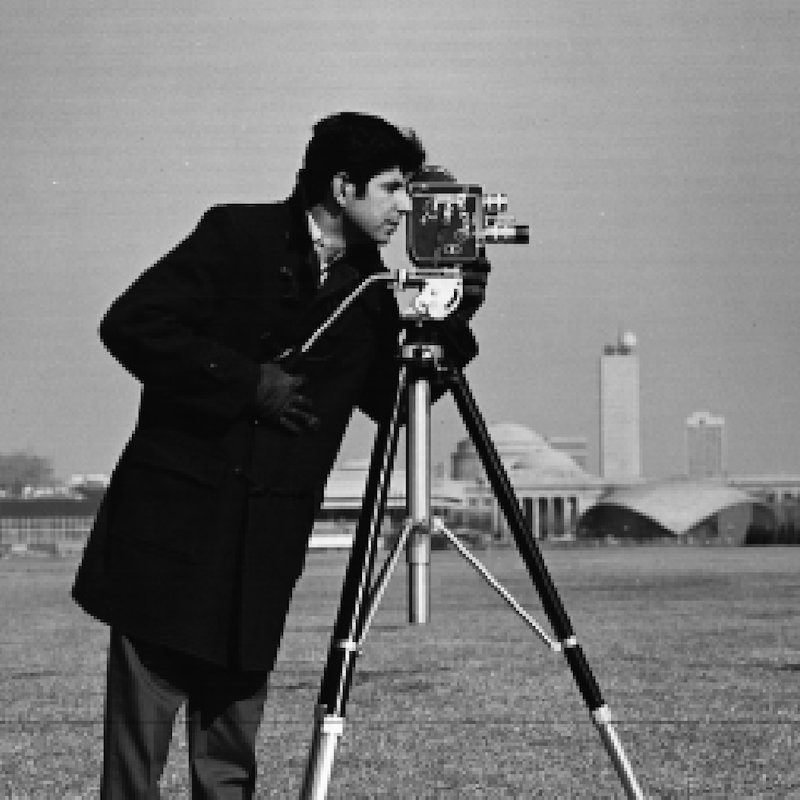
\includegraphics[width=0.4\columnwidth]{images/salt_pepper_origin.jpg}
    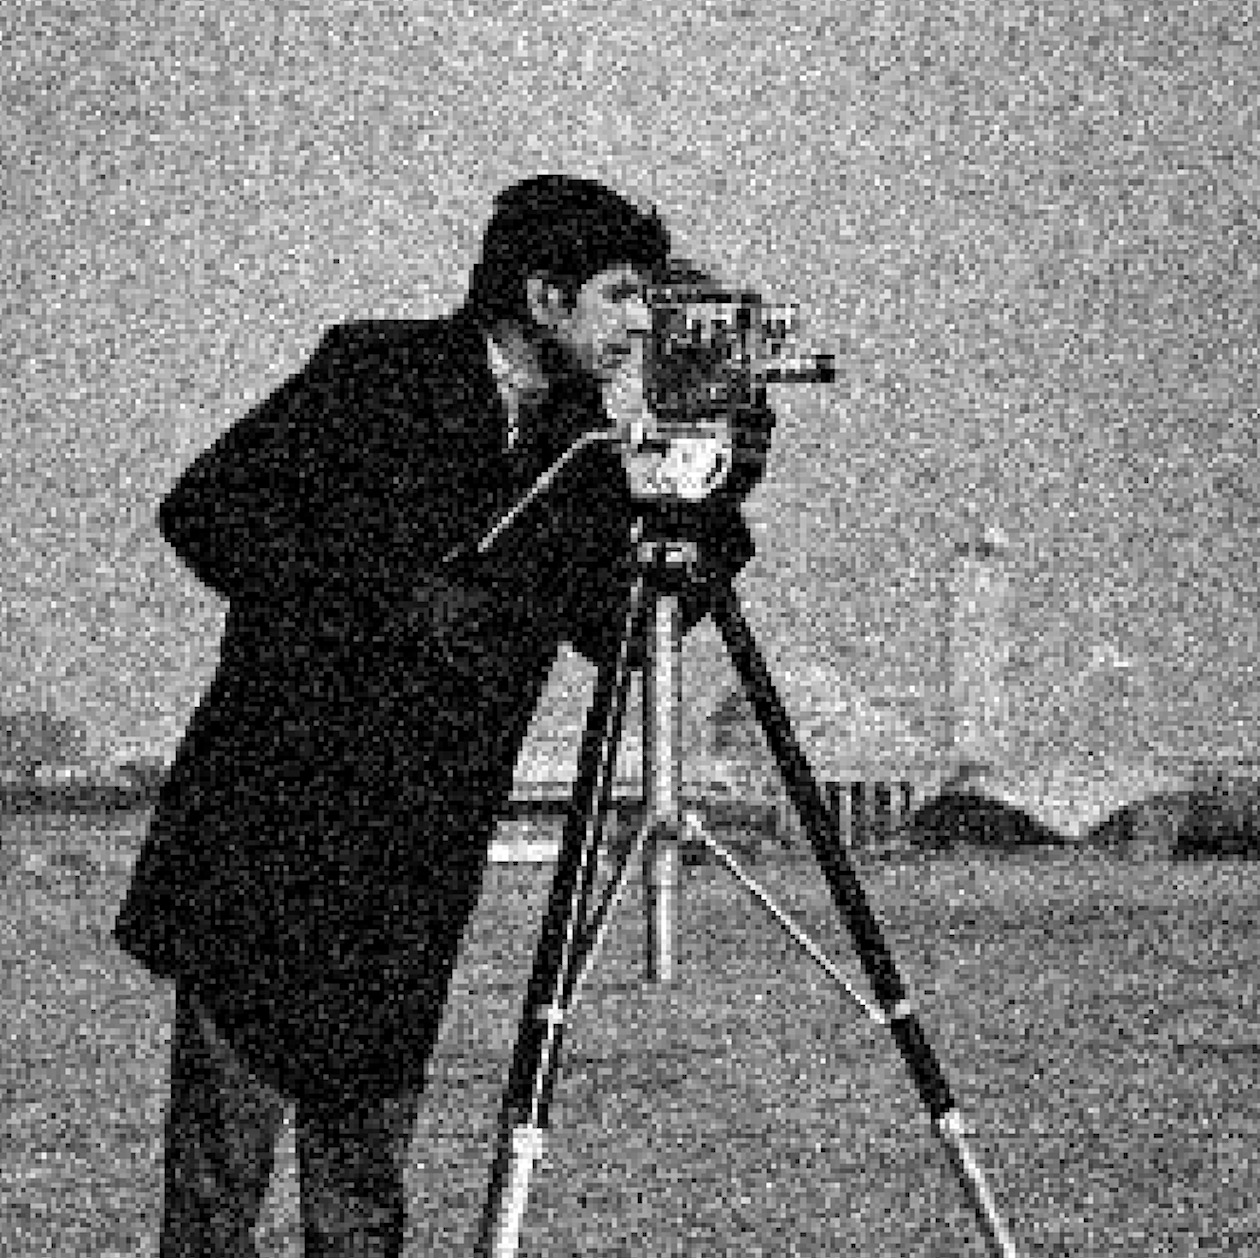
\includegraphics[width=0.4\columnwidth]{images/gaussian_noise.jpg}
	\caption{Original image (left column) and gaussian noise (right column).}
	\label{fig:gaussian_noise}
\end{figure}

%%
\textbf{Quantization Noise}, also called uniform noise, during acquisition process, when pixels of a sensed image are quantized into a number of discrete levels to perform image digitalization, quantization noise can appear. The values of quantization noise often follows approximately a uniform distribution. The probability density function $p$ of a continuous uniform random variable t is given by: 
 
\begin{equation}
    p(t)= 
\begin{cases}
    \frac{1}{b-a}, & \text{for } a \leq t \leq b \\
    0,              & \text{otherwise}
\end{cases}
\end{equation}

where a and b are the minimum and maximum values of uniform random variable $t$ respectively, the mean $\mu$ and the variance $\sigma$ of the probability density function is calculated as follows:

\begin{equation}
\mu = \frac{a+b}{2} 
\end{equation}

\begin{equation}
\sigma^{2} = \frac{(b-a)^{2}}{12}
\end{equation}

Figure~\ref{fig:quantization_noise} presents an example of image with quantization noise compared to the original image.

\begin{figure}
    \centering 
    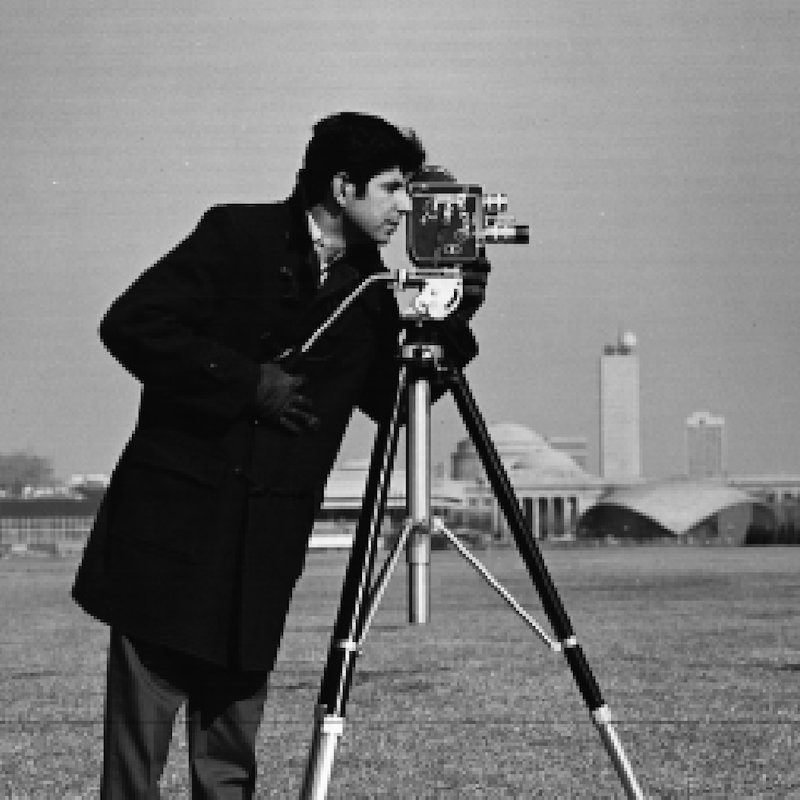
\includegraphics[width=0.4\columnwidth]{images/salt_pepper_origin.jpg}
    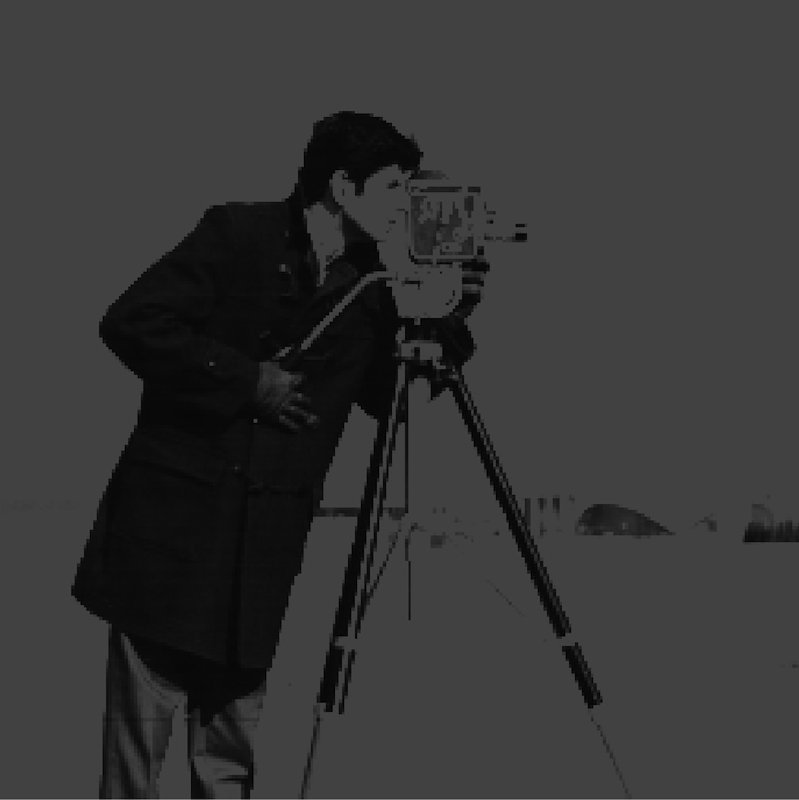
\includegraphics[width=0.4\columnwidth]{images/quantization_noise.jpg}
	\caption{Original image (left column) and quantized image to 6 bits (right column).}
	\label{fig:quantization_noise}
\end{figure}

%%
\textbf{Speckle Noise}, also called multiplicative noise: is a type of noise in which intensity values of image pixels are multiplied by undesired random values during the acquisition or transmission process. Speckle noise often happens in the cases of satellite images, medical ultrasound images or radar images, etc.

Figure~\ref{fig:speckle_noise} presents an example of image with speckle noise compared to the original image.

\begin{figure}
    \centering 
    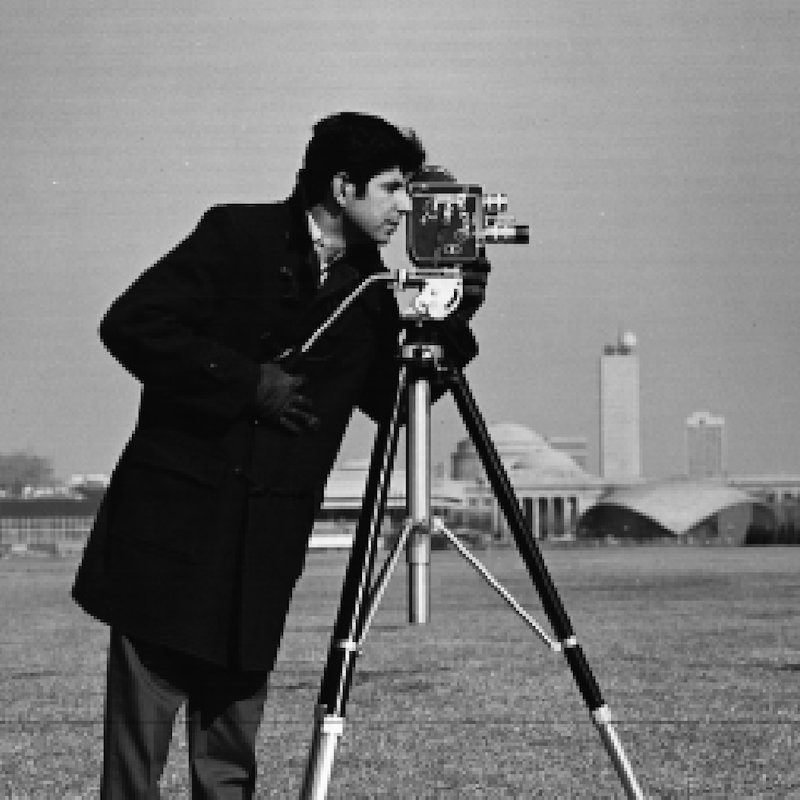
\includegraphics[width=0.4\columnwidth]{images/salt_pepper_origin.jpg}
    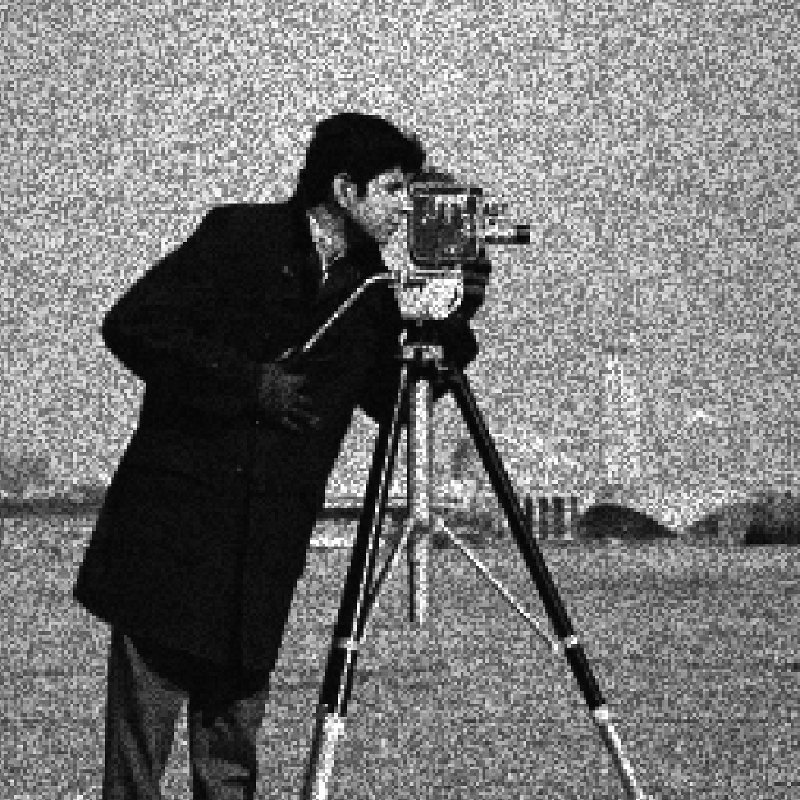
\includegraphics[width=0.4\columnwidth]{images/speckle_noise.jpg}
    \caption{Original image (left column) and image corrupted with speckle noise (right column).}
    \label{fig:speckle_noise}
\end{figure}

%%%
\subsection{Noise Removal}

Noise removal (or denoising) is a very challenging problem in image processing. It is a process to remove noise from the image and rebuild the original image in the best quality. In modern digital image processing, image denoising is a hard problem which is used in many application areas such as Optical Character Recognition (OCR), image compression, image enhancement or image segmentation, etc.

Although image denoising techniques aim at removing noise from images, they should satisfy the following objectives~\cite{liu2008automatic}:

\begin{itemize}
\item Image edges should be well preserved
\item Image details should not be lost
\item Noise from flat regions should be removed totally
\item Image global contrast should be well kept
\item No artifacts should be added in the denoised image
\end{itemize}

With these objectives, image denoising algorithms usually follows two main steps, namely types of noise recognition and noise parameterization based on recognized noise. In the internship, we are going to apply fundamental image denoising methods to improve noisy images of SWARMS project.

%%%%
\section{Report organization}

This report contains 5 chapters as follows:

\begin{itemize}
\item Chapter \ref{chapter_1}: Introduction \\
	This chapter presents context and problematic of the internship topic. 
\item Chapter \ref{chapter_2}: State of the art \\
	This chapter presents relevant research works about noise removal in digital images.
\item Chapter \ref{chapter_3}: Contribution \\
	This chapter presents studied methods in this internship to solve noise removal problem, including Median filter, Average filter, Gaussian filter and Wiener filter. 
\item Chapter \ref{chapter_4}: Results \\
	This chapter presents the results of studied methods and an analysis of these results to choose an efficient method for SWARMS project.
\item Chapter \ref{chapter_5}: Conclusion \\
	This chapter gives a conclusion about the methods and results obtained in this internship to solve the problematic. Possible future directions are also discussed. 
\end{itemize}
